\documentclass{beamer}

% Copyright 2004      by Till Tantau  <tantau@users.sourceforge.net>.
%       and 2005-2006 by Jorg Cassens <jorg.cassens@idi.ntnu.no>
%
% In principle, this file can be redistributed and/or modified under
% the terms of the GNU Public License, version 2.
%
% However, this file is supposed to be a template to be modified
% for your own needs. For this reason, if you use this file as a
% template and not specifically distribute it as part of a another
% package/program, I grant the extra permission to freely copy and
% modify this file as you see fit and even to delete this copyright
% notice.

% Describing beamerthemeTrondheim version 2006/08/23

% If you have more than three sections or more than three subsections in at least one section,
% you might want to use the [compress] switch. In this case, only the current (sub-) section
% is displayed in the header and not the full overview.


\mode<presentation>
{
  %\usetheme{Trondheim}
  \usetheme[blue,compress]{Trondheim}
%  \usetheme{Warsaw}

  \usefonttheme[onlymath]{serif}
  % \useoutertheme{infolines}
  % or whatever

  \setbeamercovered{transparent}
  % or whatever (possibly just delete it)
}

\usepackage{tikz}
% you only need this when using TikZ graphics

\usepackage{multimedia}
% you probably want to comment this out if not using multimedia elements

\usepackage{hyperref}

\usepackage[english]{babel}
% or whatever

\usepackage[latin1]{inputenc}
% or whatever

\usepackage{mathptmx}
\usepackage{helvet}
\usepackage{courier}

\usepackage[T1]{fontenc}
% Or whatever. Note that the encoding and the font should match. If T1
% does not look nice, try deleting the line with the fontenc.

\title % (optional, use only with long paper titles)
{Unofficial NTNU ``Scientific'' Theme for Beamer}

% \subtitle
% {Include Only If Paper Has a Subtitle}

\author{J\"{o}rg Cassens}

% Till Tantau\author{{1} \and
% J\"{o}rg Cassens\inst{2}

\institute[NTNU] % (optional, but mostly needed)
{Norwegian University of Science and Technology}
% - Use the \inst command only if there are several affiliations.
% - Keep it simple, no one is interested in your street address.


\date[] % (optional, should be abbreviation of conference name)
{}
% - Either use conference name or its abbreviation.
% - Not really informative to the audience, more for people (including
%   yourself) who are reading the slides online

\subject{Beamer}
% This is only inserted into the PDF information catalog. Can be left
% out.

% Delete this, if you do not want the table of contents to pop up at
% the beginning of each subsection:
% \AtBeginSubsection[]
% {
%   \begin{frame}<beamer>
%     \frametitle{Outline}
%     \tableofcontents[currentsection,currentsubsection]
%   \end{frame}
% }

\begin{document}

\begin{frame}
  \titlepage
\end{frame}

\section{Introduction}

\begin{frame}
  \frametitle{Why}

  Why use \LaTeX, when there are specialized presentations tools (OpenOffice.org Impress, Keynote, PowerPoint) available?

  \begin{itemize}
    \item{Look: The layout of mathematical formulas and program text is much nicer\ldots not to speak from ligatures in ``ordinary'' text}
    \item{Reuse of material: Going from a paper to a presentation is easy -- just use the same ``codebase''}
    \item{Portable solution: You can use whichever operating system you like}
    \item{Durable solution: usually even very old \LaTeX code can be typeset with modern installations}
  \end{itemize}

\end{frame}

\section{Cool Stuff}

\begin{frame}
  \frametitle{Mathematics}

  \begin{example}
    \begin{equation}
      \mathit{Hamming} (X,Y) = \sum_{i=1}^{l} f (x_{i}, y_{i})
    \end{equation}
  \end{example}

with $f(x,y)$ defined as follows:

  \begin{definition}
    \begin{equation}
      f(x,y)= \left\{ \begin{array}{ll}
          0 & \mbox{iff $|x-y| \leq \epsilon_{h}$,} \\
          1 & \mbox{else.}      \\
        \end{array}
      \right.
    \end{equation}
  \end{definition}

\end{frame}

\begin{frame}
  \frametitle{Piecewise Text Modification}

  \onslide<1>
    Shown on first slide.
  \onslide<2>
    Shown on second slide.
  \onslide<1>
    Shown on first slide.
    \begin{itemize}
  \onslide<2-3>
        \item Shown on the second and the third slide.
  \onslide+<3->
        \item Shown from slide 3 on.
    \end{itemize}
    Shown from slide 3 on.
  \onslide
    Shown on all slides.

  \onslide<4>
    \alert<4>{You get fine-grain control over which elements are visible at each time.}

\end{frame}

\begin{frame}
  \frametitle{Using Ti\textit{k}Z for Drawings}

  % The stuff for this slide is taken from the PGF Manual

  % New example using TikZ

    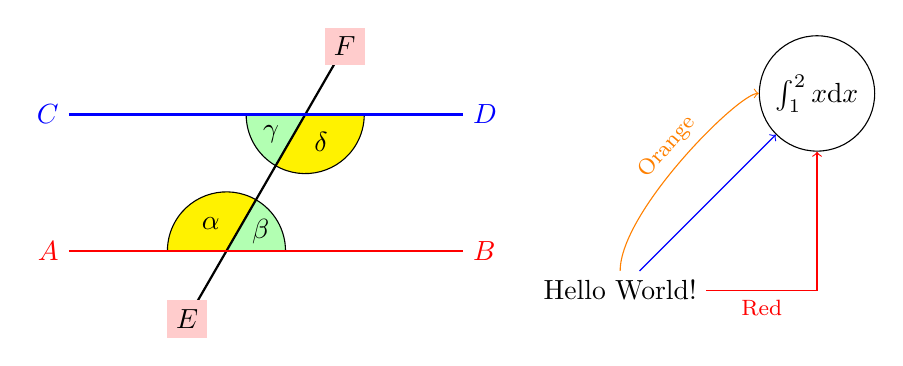
\begin{tikzpicture}
      \draw[fill=yellow] (0,0) -- (60:.75cm) arc (60:180:.75cm);
      \draw(120:0.4cm) node {$\alpha$};
      \draw[fill=green!30] (0,0) -- (right:.75cm) arc (0:60:.75cm);
      \draw(30:0.5cm) node {$\beta$};
      \begin{scope}[shift={(60:2cm)}]
        \draw[fill=green!30] (0,0) -- (180:.75cm) arc (180:240:.75cm);
        \draw (30:-0.5cm) node {$\gamma$};
        \draw[fill=yellow] (0,0) -- (240:.75cm) arc (240:360:.75cm);
        \draw (-60:0.4cm) node {$\delta$};
      \end{scope}
      \begin{scope}[thick]
        \draw (60:-1cm) node[fill=red!20] {$E$} -- (60:3cm) node[fill=red!20] {$F$};
        \draw[red] (-2,0) node[left] {$A$} -- (3,0) node[right]{$B$};
        \draw[blue,shift={(60:2cm)}] (-3,0) node[left] {$C$} -- (2,0) node[right]{$D$};
      \end{scope}
      \path (5,-0.5) node (x) {Hello World!}
      (7.5,2) node[circle,draw](y) {$\int_1^2 x \mathrm d x$};
      \draw[->,blue] (x) -- (y);
      \draw[->,red] (x) -| node[near start,below] {\footnotesize Red} (y);
      \draw[->,orange] (x) .. controls +(up:1cm) and +(left:1cm) .. node[above,sloped] {\footnotesize Orange} (y);
    \end{tikzpicture}

%   % Old example demonstrating PGF capabilities

%   \begin{pgfpicture}{0cm}{0cm}{5cm}{2cm}
%     \pgfputat{\pgfxy(1,1)}{\pgfbox[center,center]{Hi!}}
%     \pgfcircle[stroke]{\pgfxy(1,1)}{0.5cm}
%     \pgfline{\pgfxy(1.5,1)}{\pgfxy(2.2,1)}
%      \pgfputat{\pgfxy(3,1)}{
%      \begin{pgfrotateby}{\pgfdegree{30}}
%        \pgfbox[center,center]{$\int_0^\infty xdx$}
%      \end{pgfrotateby}}
%     \pgfcircle[stroke]{\pgfxy(3,1)}{0.75cm}
%
%     \pgfmoveto{\pgfxy(5,1)}
%     \pgfcurveto{\pgfxy(6,0.5)}{\pgfxy(6,1.5)}{\pgfxy(8,1)}
%     \pgfstroke
%     \pgfsetdash{{3pt}{3pt}}{0pt}
%     \pgfmoveto{\pgfxy(5,1)}
%     \pgflineto{\pgfxy(6,0.5)}
%     \pgflineto{\pgfxy(6,1.5)}
%     \pgflineto{\pgfxy(7,1)}
%     \pgfstroke
%
%     \pgfmoveto{\pgfxy(9,1)}
%     \pgfcurveto{\pgfxy(9,0)}{\pgfxy(10,0)}{\pgfxy(10,1)}
%     \pgfcurveto{\pgfxy(10,2)}{\pgfxy(9,2)}{\pgfxy(9,1)}
%     \pgfclosepath
%     \pgffill
%   \end{pgfpicture}

  \vspace*{.5cm}

  Take a look into the \href{http://story.idi.ntnu.no/~cassens/download/latex/beamer/beamerTrondheimExample.tex}{\alert{souce code}} to see how this is done.

\end{frame}

\begin{frame}
  \frametitle{Including Movies}

  \pgfdeclareimage[interpolate=true,width=.45\textwidth]{ccpict}{Building_On_The_Past}

  \begin{center}
    \movie[poster,externalviewer,label=ccmovie]{\pgfuseimage{ccpict}}{Building_On_The_Past.mpg}
  \end{center}

  {\small
  To watch the movie in an external player application, click on the picture above.% or \hyperlinkmovie{ccmovie}{\beamerbutton{press this button}}.

  The video is not included in the distribution of this PDF. To watch it, just \href{http://story.idi.ntnu.no/~cassens/download/latex/beamer/Building_On_The_Past.mpg}{\alert{download it}} and place it in the same directory as this PDF file.
  }

  {\tiny Video published under the \href{http://creativecommons.org/}{\alert{CreativeCommons}} \href{http://creativecommons.org/licenses/by-nc/1.0/}{\alert{``Attribution NonCommercial''}} license by \href{http://justincone.com/main.html}{\alert{Justin Cone}.}}

\end{frame}

\section{Coloured Boxes}

\subsection{Alerts and Examples}

\begin{frame}
  \frametitle{Alert}

  Alert boxes direct the attention of the audience.

  \begin{alertblock}{Lorem Ipsum}
    ``Lorem ipsum dolor sit amet, consectetuer.''
  \end{alertblock}

  Non eram nescius, Brute, cum, quae summis ingeniis exquisitaque doctrina philosophi Graeco sermone tractavissent, ea Latinis litteris mandaremus, fore ut hic noster labor in varias reprehensiones incurreret.

  Nam quibusdam, et iis quidem non admodum indoctis, totum hoc displicet philosophari.
\end{frame}

\begin{frame}
  \frametitle{Exampleblock}

  Examples are also highlighted in a different colour, making them less obstrusive.

  \begin{example}
    ``Laoreet dolore magna ali quam erat volutprat.''
  \end{example}

  You can also use a custom title:

  \begin{exampleblock}{Comodo consequat}
    ``Ut wisi enim ad mi nim veniam, quis nostrud exerci.''
  \end{exampleblock}

\end{frame}

\subsection{Theorems and Definitons}

\begin{frame}
  \frametitle{Theorem}

  Theorems and definitions come in their own coloured boxes. A theorem:

  \begin{theorem}
    ``Lorem ipsum dolor sit amet, consectetuer.''
  \end{theorem}

  And a definition:

  \begin{definition}
    ``Laoreet dolore magna ali quam erat volutprat.''
  \end{definition}

\end{frame}


\subsection{Other Boxes}

\begin{frame}
  \frametitle{Block}

  Blue boxes can also be used for other content you want to highlight.

  \begin{block}{Comodo consequat}
    ``Laoreet dolore magna ali quam erat volutprat.''
  \end{block}

  You can also create boxes with no header.

  \begin{block}{}
    ``Ut wisi enim ad mi nim veniam, quis nostrud exerci.''
  \end{block}

\end{frame}

\begin{frame}
  \frametitle{Beamercolorbox}

  Simple colored boxes are the least decorated way to draw attention to certain areas:\newline

  \begin{beamercolorbox}[sep=0.5em]{block title}
    ``Lorem ipsum dolor sit amet, consectetuer.''
  \end{beamercolorbox}

  \vspace*{.5cm}

  Quidam autem non tam id reprehendunt, si remissius agatur, sed tantum studium tamque multam operam ponendam in eo non arbitrantur.

  Erunt etiam, et ii quidem eruditi Graecis litteris, contemnentes Latinas, qui se dicant in Graecis legendis operam malle consumere. Postremo aliquos futuros suspicor, qui me ad alias litteras vocent, genus hoc scribendi, etsi sit elegans, personae tamen et dignitatis esse negent.

\end{frame}

\section{Conclusions}

\begin{frame}
  \frametitle{Options}

  \begin{itemize}
    \item{\textbf{Background colour:} [blue|sand] set the background colour accordingly}
    \item{\textbf{Logo:} [nynorsk|bokmaal|mylogo|nologo] use one of the norwegian versions of the logo on the titlepage, your logo, or no logo at all}
    \item{\textbf{Page numbers:} [numbers] will include the number of the current slide in the footer}
    \item{\textbf{Section overview:} [compress|minmal] will only show the current section and subsection in the header or no section overview at all}
  \end{itemize}

  \begin{example}
   $\backslash$usetheme[blue,compress,numbers,bokmaal]\{Trondheim\}
  \end{example}
\end{frame}

\begin{frame}
  \frametitle{Conclusions}

  \begin{itemize}
    \item{Theme based on Warsaw theme that comes with Beamer}
    \item{It is in my oppinion better suited for scientific talks than the official NTNU style}
    \item{The colours used in this theme are based on the offical ``NTNU blue'' plus darker and lighter variants}
    \item{The compress switch is useful if you are having (too) many (sub-) sections}
    \item{Options sand and blue for a slightly coloured background}
    \item{Feedback appreciated: \href{mailto:jorg.cassens@idi.ntnu.no}{\texttt{jorg.cassens@idi.ntnu.no}}}
    \item{If you still want to use a theme which copies the official design: H\aa vard Berland has created a nice \href{http://www.math.ntnu.no/~berland/ntnubeamer/}{\alert{Beamer theme}}}
  \end{itemize}
\end{frame}

\end{document}
